\documentclass[10pt]{beamer}

%% Based on the original theme by Matthias Vogelgesang

\usetheme[progressbar=frametitle]{metropolis}
\usepackage{appendixnumberbeamer}

\usepackage{booktabs}
\usepackage[scale=2]{ccicons}

\usepackage{pgfplots}
\usepgfplotslibrary{dateplot}

\usepackage{xspace}
\newcommand{\themename}{\textbf{\textsc{metropolis}}\xspace}

%%%%%%%%%%%%%%%%%%%%%%%%%%%%
%% UNCC Theme Adjustments %%
%%%%%%%%%%%%%%%%%%%%%%%%%%%%
\definecolor{CanvasBG}{HTML}{FAFAFA}

% From the official style guide
\definecolor{UnccGreen}{HTML}{00703C}
\definecolor{UnccGold}{HTML}{B3A369}
\definecolor{UnccLightGreen}{HTML}{C3D7A4}
\definecolor{UnccYellow}{HTML}{F0CB00}
\definecolor{UnccOrange}{HTML}{F3901D}
\definecolor{UnccLightYellow}{HTML}{FFF6DC}
\definecolor{UnccBlue}{HTML}{00728F}
\definecolor{UnccPink}{HTML}{DE3A6E}
\definecolor{White}{HTML}{FFFFFF}
\definecolor{LightGray}{HTML}{DDDDDD}

% Supporting Color Palette
\definecolor{WarmGray}{HTML}{696158}
\definecolor{StoneGray}{HTML}{717C7D}
\definecolor{DarkGreen}{HTML}{2C5234}
\definecolor{LightGreen}{HTML}{509E2F}
\definecolor{BrightGold}{HTML}{F0CB00}

% Screamers
\definecolor{Royal}{HTML}{72246C}
\definecolor{Ocean}{HTML}{006BA6}
\definecolor{Flash}{HTML}{B52555}
\definecolor{Citrus}{HTML}{FFB81C}
\definecolor{Spring}{HTML}{CEDC00}

% Serenity
\definecolor{Garden}{HTML}{B7CE95}
\definecolor{Sand}{HTML}{F0E991}
\definecolor{Bloom}{HTML}{F1E6B2}
\definecolor{Clay}{HTML}{B7B09C}
\definecolor{Cloud}{HTML}{BAC5B9}

% Set colors here
\setbeamercolor{frametitle}{bg=UnccGreen}
\setbeamercolor{progress bar}{bg=BrightGold, fg=UnccGreen}
\setbeamercolor{alerted text}{fg=Flash}

\setbeamercolor{block title}{bg=LightGreen, fg=White}
\setbeamercolor{block title example}{bg=Ocean, fg=White}
\setbeamercolor{block title alerted}{bg=Citrus, fg=White}
\setbeamercolor{block body}{bg=CanvasBG}

\metroset{titleformat=smallcaps, progressbar=foot, sectionpage=none}

\makeatletter
\setlength{\metropolis@progressinheadfoot@linewidth}{2pt}
\setlength{\metropolis@titleseparator@linewidth}{2pt}
\setlength{\metropolis@progressonsectionpage@linewidth}{2pt}
%%%%%%%%%%%%%%%%%%%%%%%%%%%%
%% UNCC Theme Adjustments %%
%%%%%%%%%%%%%%%%%%%%%%%%%%%%


\title{Antrittsvortrag}
\subtitle{Handgestenerkennung mit Entscheidungsbäumen}
% \date{\today}
\date{30.11.2020}
\author{Tom Dymel}
\institute{Forschungsprojekt und Seminar\\Technische Universität Hamburg}
% \titlegraphic{\hfill\includegraphics[height=1.5cm]{logo.pdf}}

\begin{document}

\maketitle

\section{Motivation}
\begin{frame}{Motivation}
% TODO: Raussuchen, was die jeweiligen Leute gemacht haben und wie gut das ist
\begin{itemize}
    \item Zuverlässige Gestenerkennung auf Micro-Controller
    \item Preiswertes Modul
    \item Echtzeit-Evaluierung 
    \item Vorherige Ansätze:
    \begin{itemize}
        \item FFNN (Engelhardt, Kubik, Giese)
        \item RNN (Klisch, Engelhardt)
    \end{itemize}
    \item Entscheidungsbäume potentiell effizienter
\end{itemize}
\end{frame}

\section{Optische Handgestenerkennung}
%Kurz!
\begin{frame}{Optische Handgestenerkennung}
\begin{figure}
    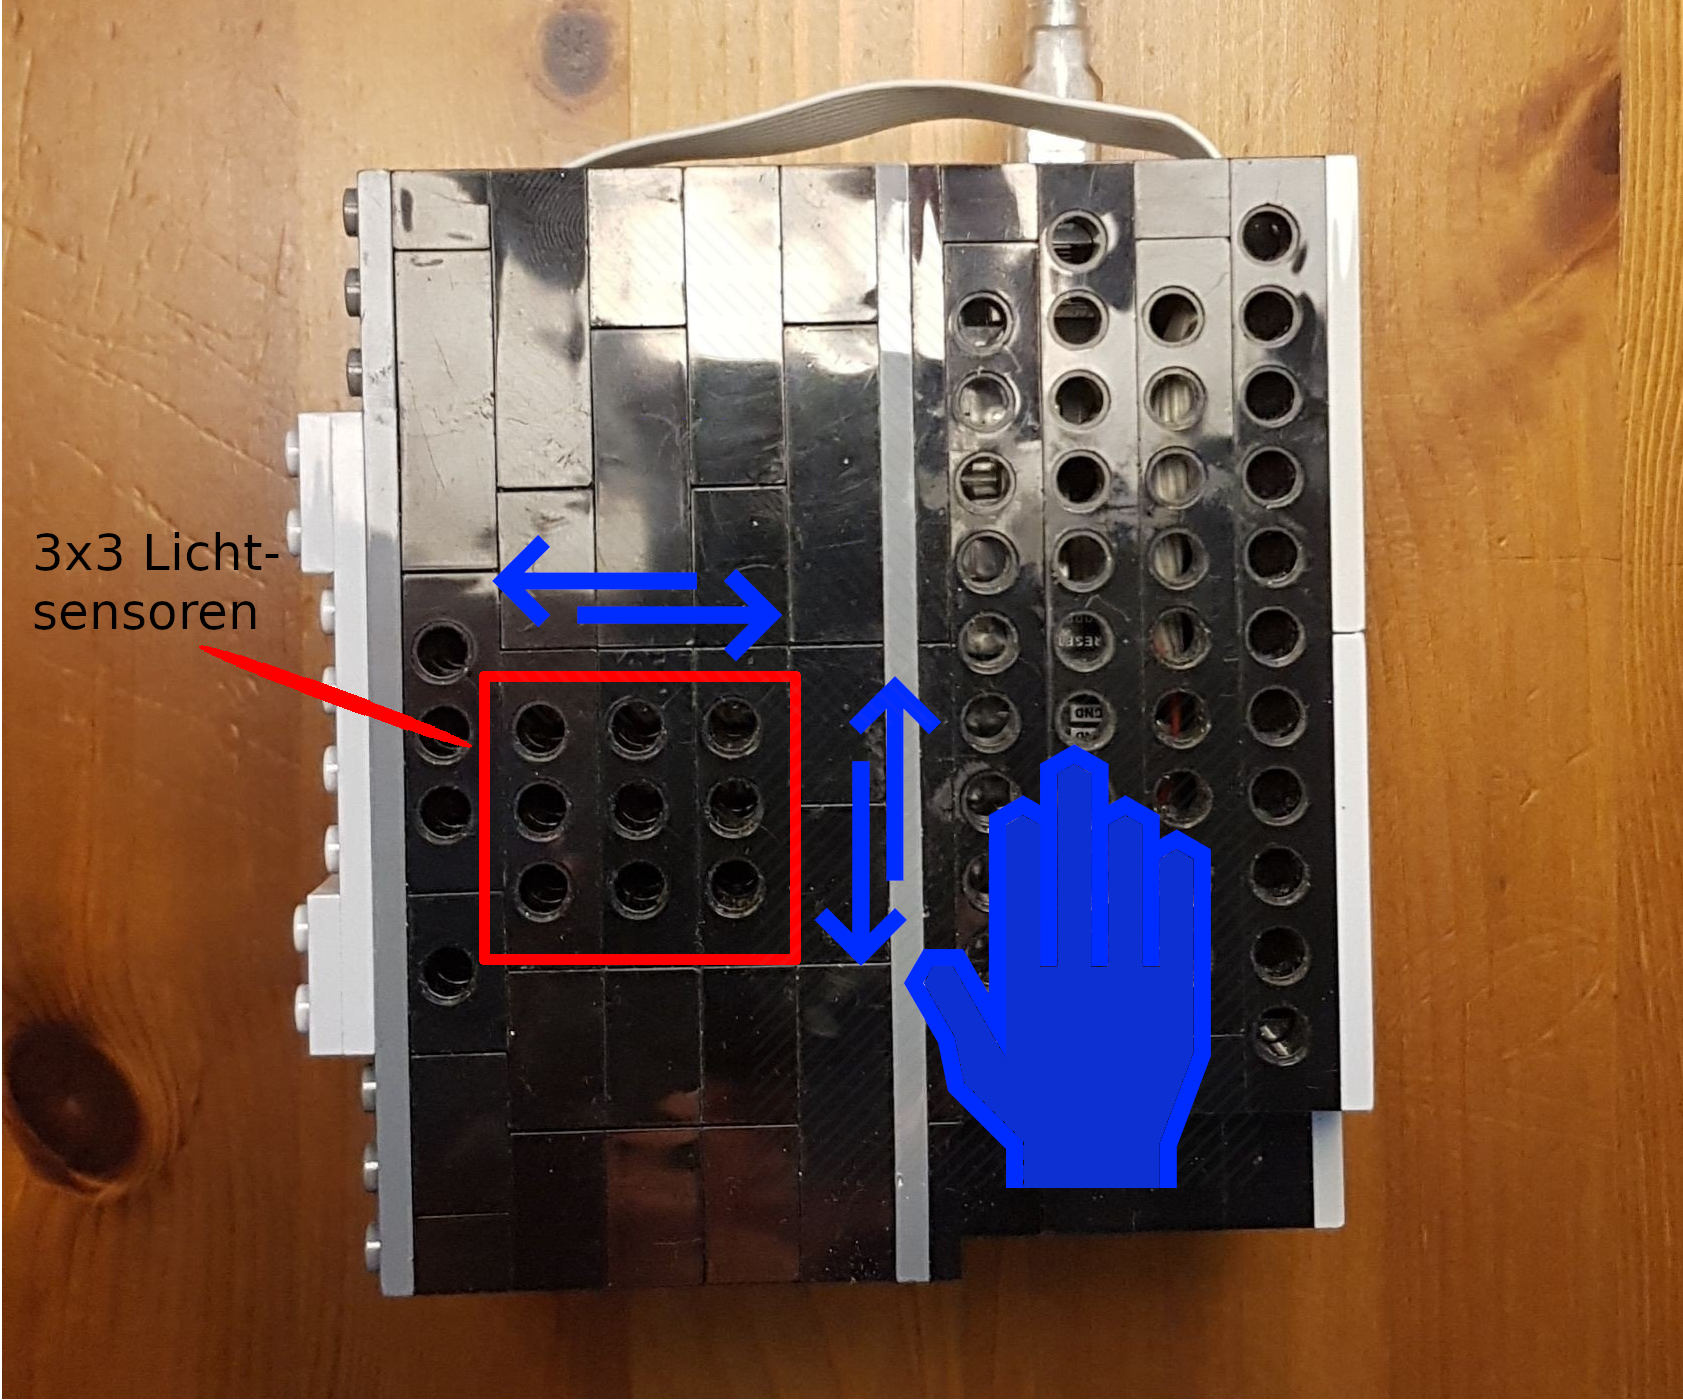
\includegraphics[width=0.9\linewidth]{aufgabe.png}
  \end{figure}
\end{frame}

\section{Entscheidungsbäume}
\begin{frame}{Entscheidungsbäume}
\begin{figure}
    \centering
    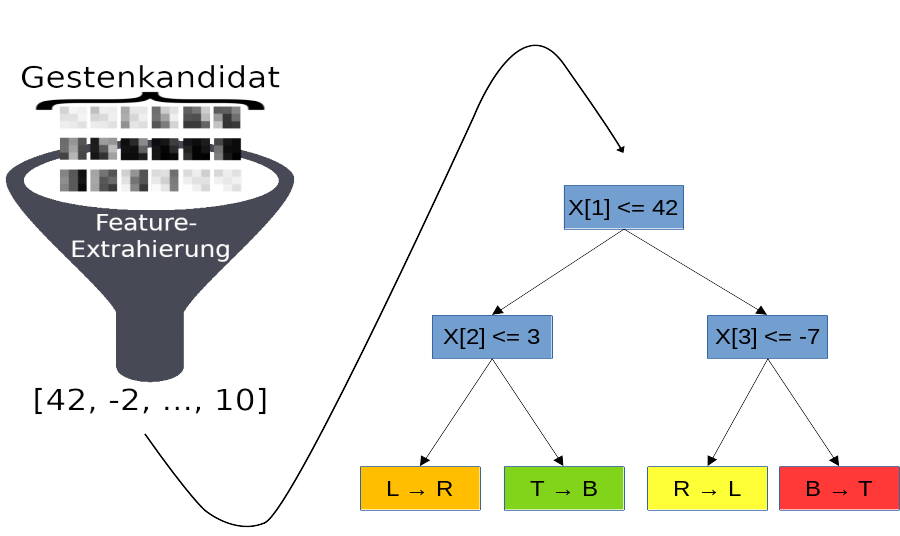
\includegraphics[width=\linewidth]{process_draw.png}
\end{figure}
\end{frame}

\section{Momentaner Stand}
\begin{frame}{Momentaner Stand}
\begin{itemize}
    \item 28 verschiedene Features untersucht
    \item 5 verschiedene Ensamble Methoden untersucht
    \item Aktuell: Schwerpunktverteilung über 5 Zeitfenster
    \item Aktuell: RandomForest - Trainiert mit Scikit-Learn
    \item Trainingsdaten von Kubik und Feng's 3x3- und 4x4-Pixel-Kamera
    \item Testdaten von Klisch
\end{itemize}
\end{frame}

\begin{frame}{Momentaner Stand - Schwerpunktverteilung}
\begin{figure}
    \begin{minipage}[c]{0.5\linewidth}
        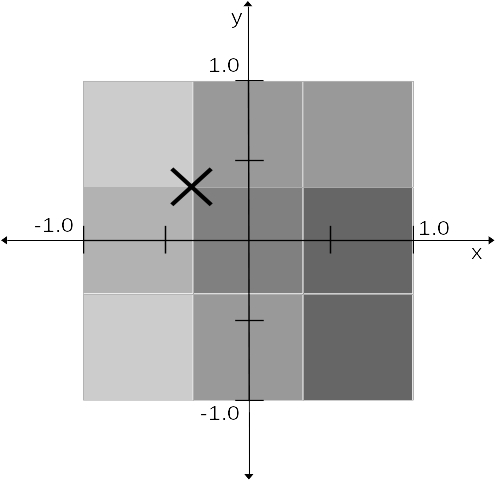
\includegraphics[width=\linewidth]{schwerpunkt_ansatz.jpg}
    \end{minipage}
    \hfill
    \begin{minipage}[c]{0.3\linewidth}
        $\begin{pmatrix}
            p_{00} & p_{01} & p_{02}\\
            p_{10} & p_{11} & p_{12}\\
            p_{20} & p_{21} & p_{22}
        \end{pmatrix}$
        \\\\\\
        $P = \sum_{i,j} p_{i,j}$
        \\\\
        $X_s = \frac{\sum_{i=0}^{2} p_{i,2} - \sum_{i=0}^{2} p_{i,0}}{P}$
        \\\\
        $Y_s = \frac{\sum_{i=0}^{2} p_{0,i} - \sum_{i=0}^{2} p_{2,i}}{P}$
    \end{minipage}
\end{figure}
\begin{itemize}
    \item Komprimieren auf 5 Schwerpunkte über Durchschnitt
\end{itemize}
\end{frame}

\begin{frame}{Momentaner Stand - Schwerpunkte mit Float}
% Hier anmerken:
% Was ist mit "Worst-Case" gemeint?
% Vergleich mit der besten anderen Arbeit (Giese?)
% Anmerken, dass die beste Konfiguration mit 32KB Porgrammsize konstraint arbeitet
% und dass mit mehr bis zu 98% möglich ist
\begin{figure}
    \begin{minipage}[c]{0.49\linewidth}
        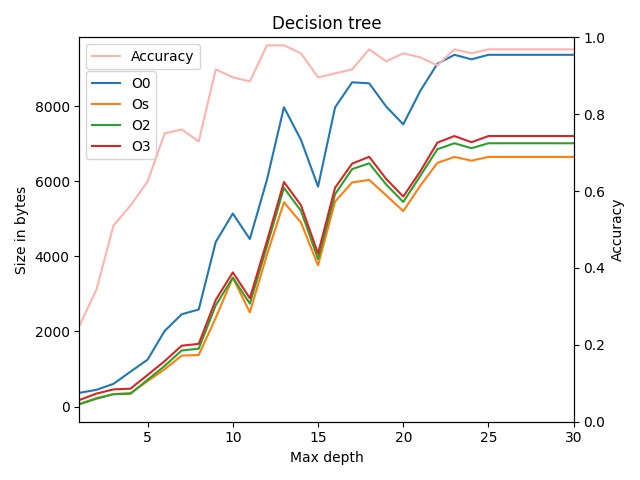
\includegraphics[width=\linewidth]{klisch_float_tree.png}
    \end{minipage}
    \hfill
    \begin{minipage}[c]{0.49\linewidth}
        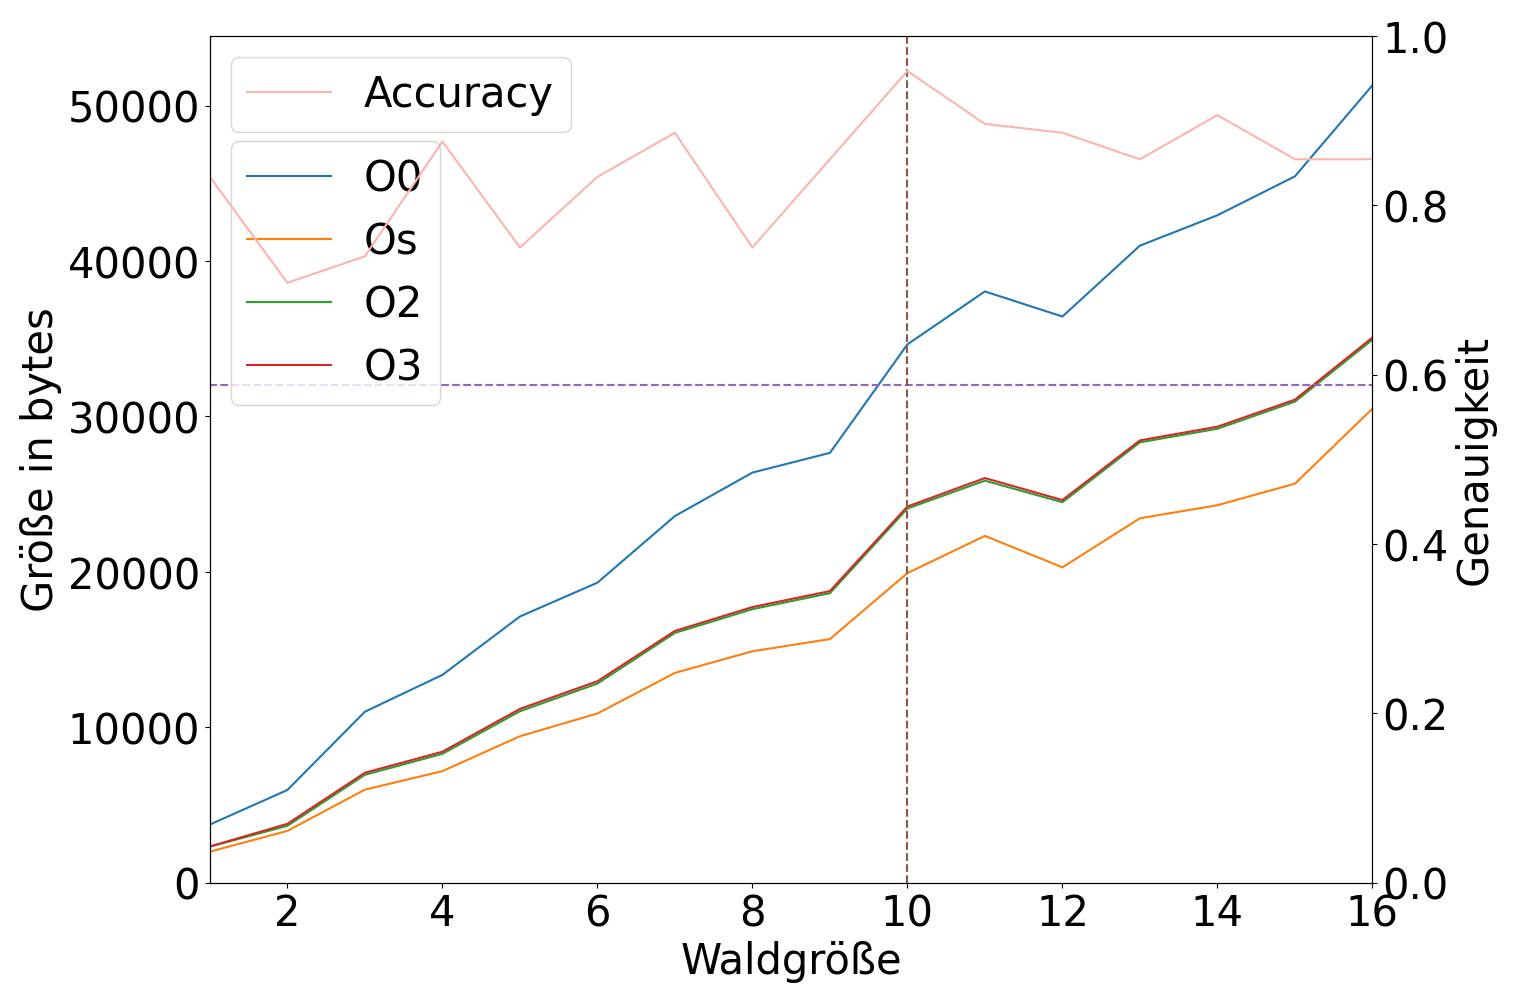
\includegraphics[width=\linewidth]{klisch_float_forest.png}
    \end{minipage}%
\end{figure}
\begin{itemize}
    \item Baum Ausführungszeit: $\leq\ $Tiefe$\ \cdot \ 4,2\ \mu s$
    \item Wald Overhead: $\leq 4\mu s$
    \item Bester Wald: 10 Bäume à 9 Max-Tiefe (95,8\% Genauigkeit)
    \begin{itemize}
        \item Größe: 22428 Bytes
        \item Ausführungszeit: $\leq 380,9\ \mu s$
    \end{itemize}
    \item Feature-Extrahierung: $\leq 483,9\ \mu s\ +\ $\#Bilder$\ \cdot \ 27,4\ \mu s$
    \item Worst-Case Gesamtausführungszeit: $\leq 3056,8\ \mu s \approx 3$ ms
\end{itemize}
\end{frame}

\begin{frame}{Momentaner Stand - Schwerpunkte mit Integer (4 Byte)}
\begin{figure}
    \begin{minipage}[c]{0.49\linewidth}
        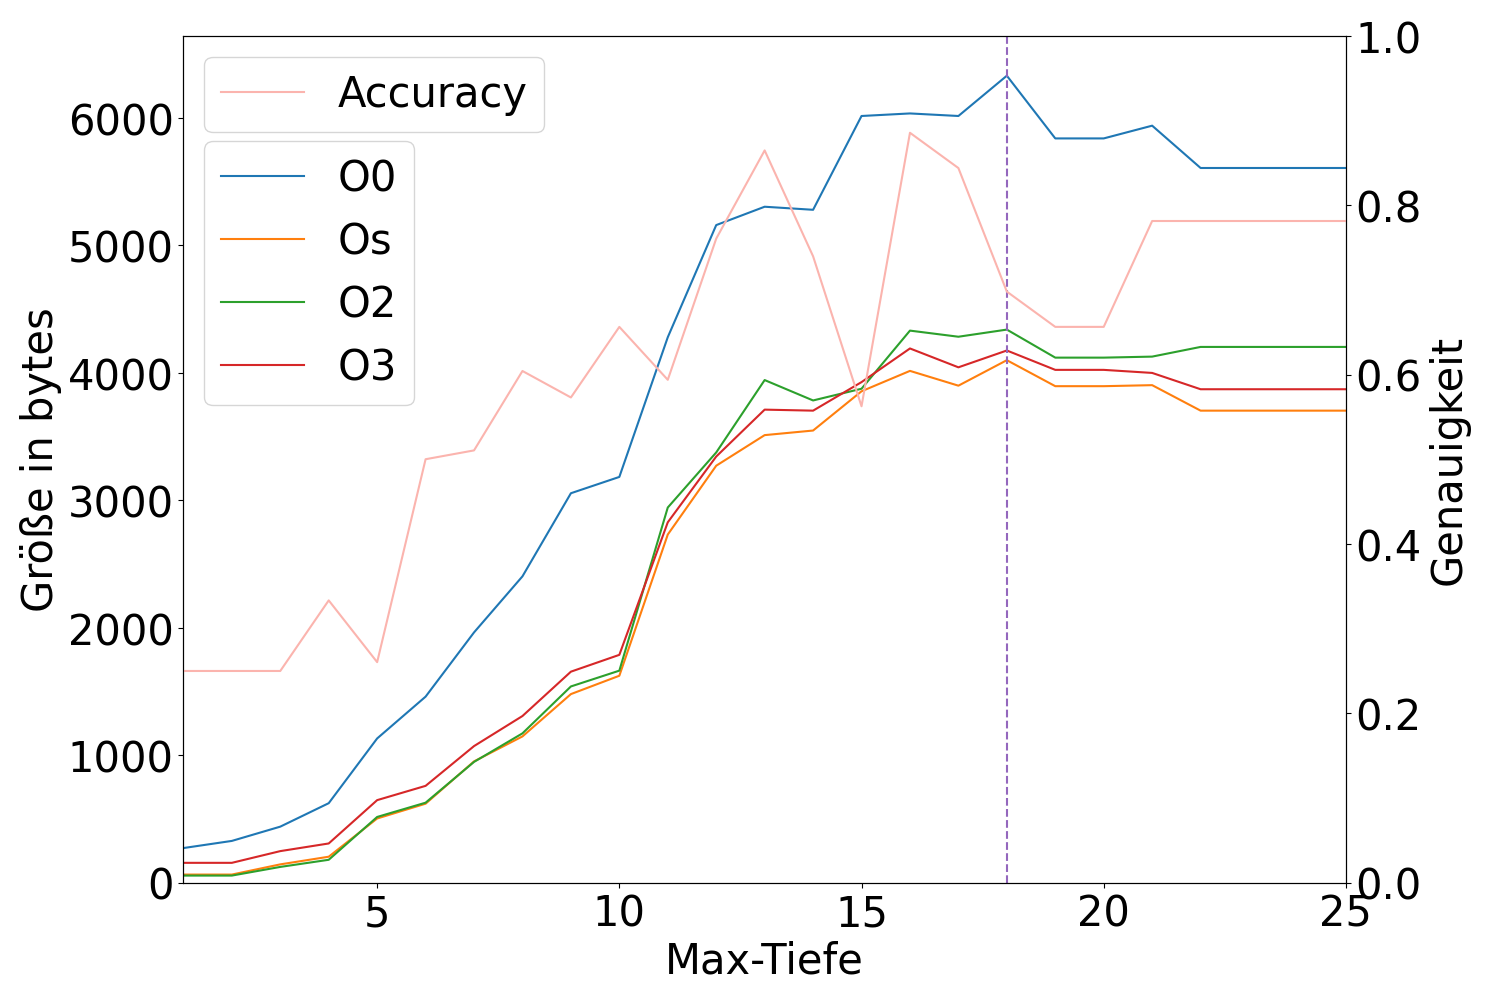
\includegraphics[width=\linewidth]{klisch_int_tree.png}
    \end{minipage}
    \hfill
    \begin{minipage}[c]{0.49\linewidth}
        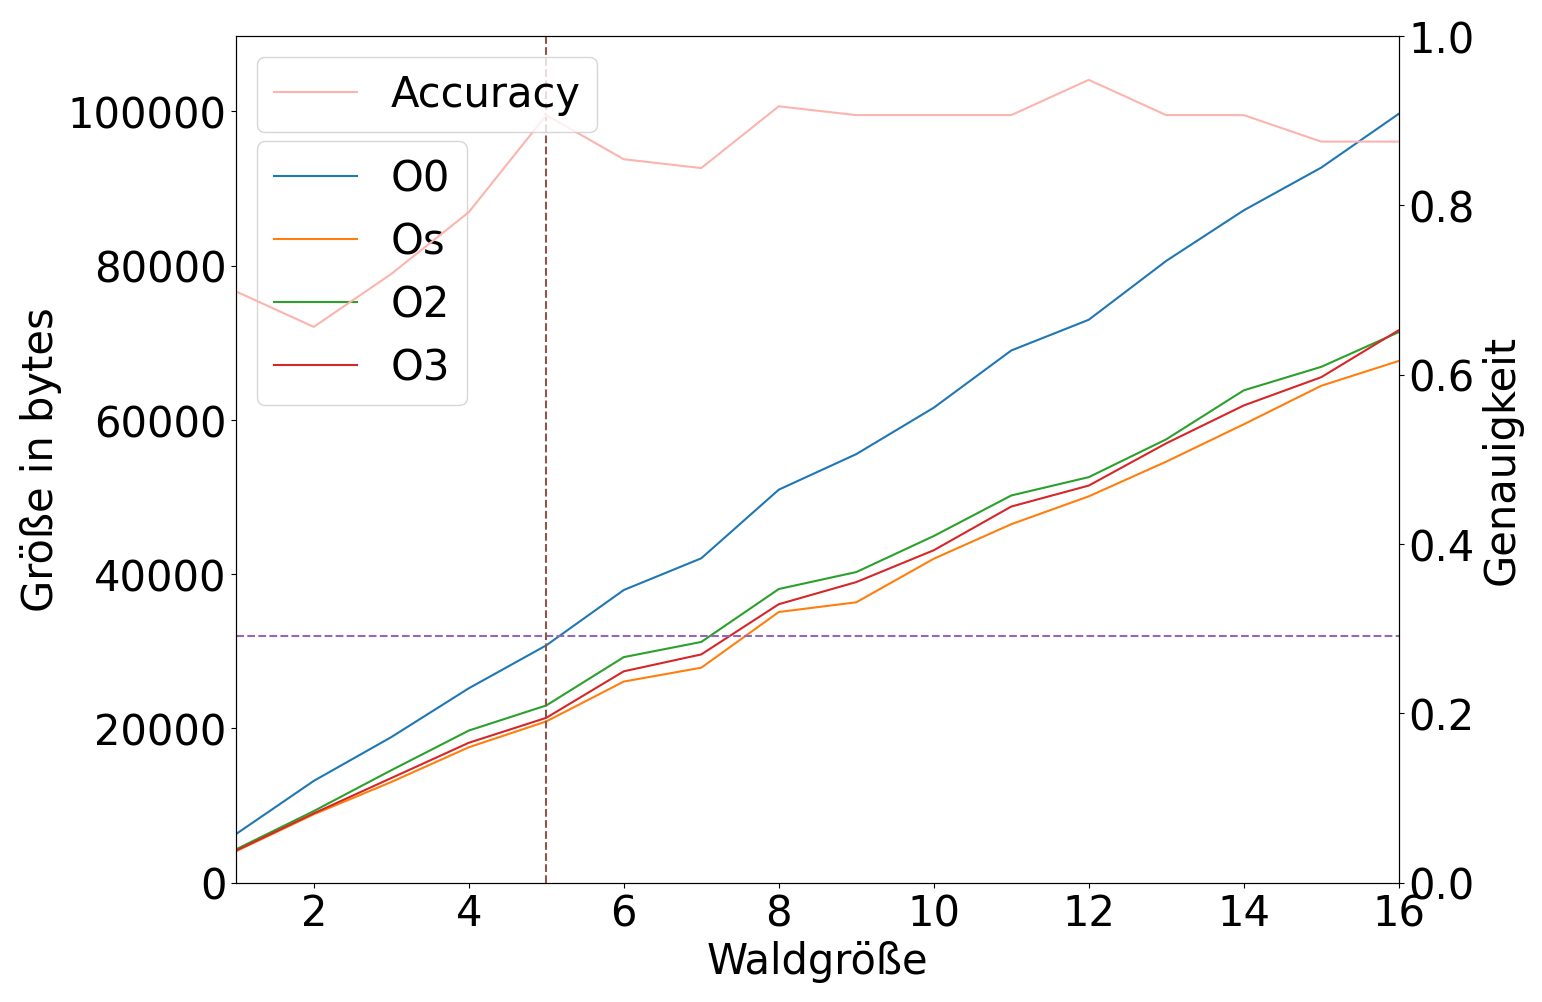
\includegraphics[width=\linewidth]{klisch_int_forest.png}
    \end{minipage}%
\end{figure}
\begin{itemize}
    \item Baum Ausführungszeit: $\leq \ $Tiefe$\ \cdot \ 0,94\ \mu s$
    \item Wald Overhead: $\leq 4\ \mu s$
    \item Bester Wald: 5 Bäume à 18 Max-Tiefe (90,6\% Genauigkeit)
    \begin{itemize}
        \item Größe: 23416 Bytes
        \item Ausführungszeit: $\leq 88,4\ \mu s$
    \end{itemize}
    \item Feature-Extrahierung: $\leq 530\ \mu s\ +\ $\#Bilder$\ \cdot \ 2,25\ \mu s$
    \item Worst-Case Gesamtausführungszeit: $\leq 798,4\ \mu s \approx 0,8$ ms
\end{itemize}
\end{frame}

\section{ToDo}
\begin{frame}{ToDo}
\begin{itemize}
    \item Weitere Entscheidungsbaumansätze evaluieren
    \item Nullgesten betrachten
    \item Robuster gegenüber Rotation ($\pm$ 30°)
    \item Robustheit gegenüber Lichtverhältnisse untersuchen
    \item Bäume verkleinern
\end{itemize}
\end{frame}

\section{Zeitplan}
\begin{frame}{Zeitplan}
\begin{figure}
    \centering
    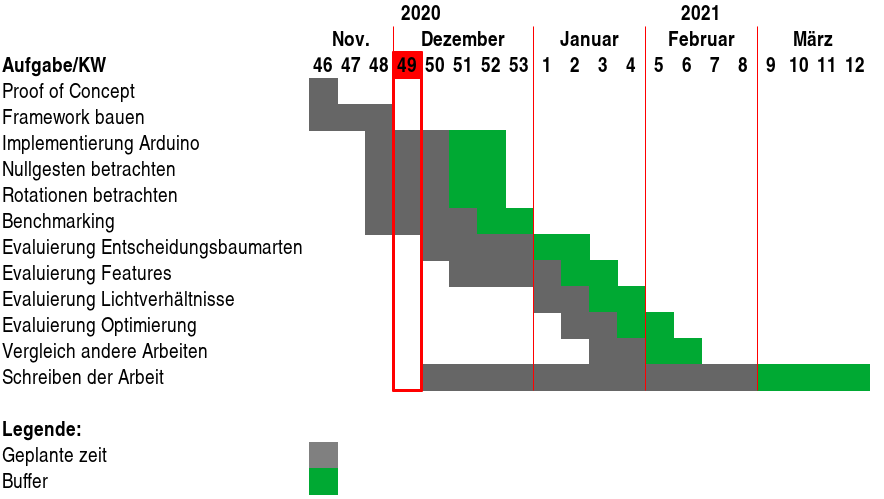
\includegraphics[width=\linewidth]{gantt_chart.png}
\end{figure}
\end{frame}
\begin{frame}[standout]
  Fragen?
\end{frame}

\end{document}
